\chapter{Applications}
\paragraph{Power-law noise}
The statistical test mentioned in the previously chapter is tested on computer generated power-law noise series.\cite{Timmer1995} the $\beta$ term in the formula $\frac{1}{f^{\beta}}$ will be referenced as k for the rest of the paper. Three values of k is chosen: $k_1=(1,3,5)$. For each $k_1$ value another set of k values is generated using the formula $k_2=(k_1-e^0,k_1-e^{-1},k_1-e^{-2},k_1-e^{-3},k_1+0,k_1+e^0,k_1+e^{-1},k_1+e^{-2},k_1+e^{-3})$. The statistical test is used on every possible pair of a value from $k_1$ and a value from $k_2$. Two power-law series is generated using each value in the pair. The series have 1,000 elements. The hypothesis will be rejected if the p values is less then 0.05. 10 iterations is done for each pair. A plot will be made for each $k_1$ value of the rejection rate of the statistical test. A NaN plot is include for each plot, that shows the rate, at which the statistical test produces NaN values. A k value difference of 1 leads in most cases to high rejection rate, with 0-1 being the only exception. Only for $k_1=5$ does NaN values occur. Power-law series with $k=5$ and 1,000 values has an entropy around 0.4. The datasets that will be examined in the rest of the paper has entropy above 0.9, so no NaN values is expected to occur.

\begin{figure}
    \centering
    \begin{subfigure}[b]{0.3\textwidth}
        \centering
        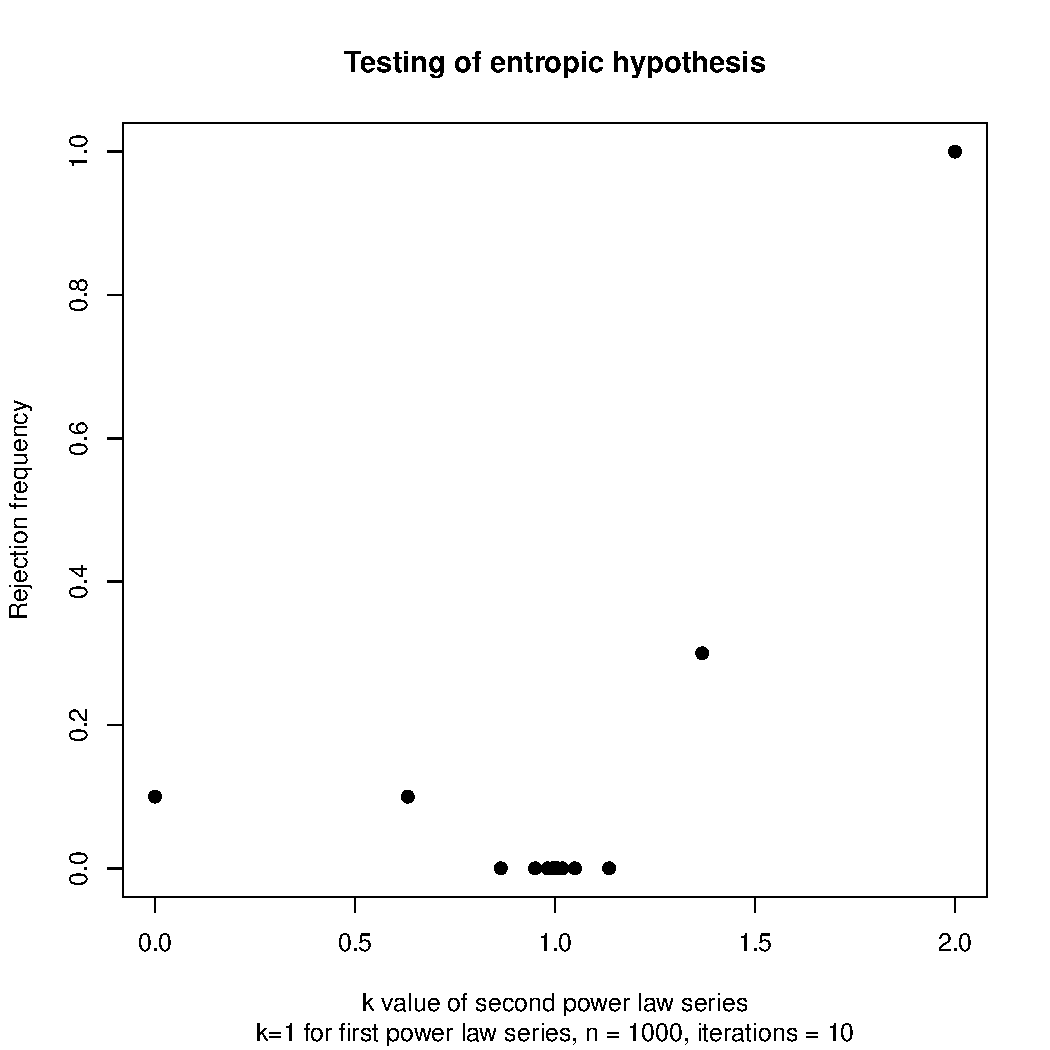
\includegraphics[height=7cm,keepaspectratio]{powerlaw/rejectionPlot,k1=1, n=1000, iterations=10.pdf}
    \end{subfigure}
    \hfill
    \begin{subfigure}[b]{0.5\textwidth}
        \centering
        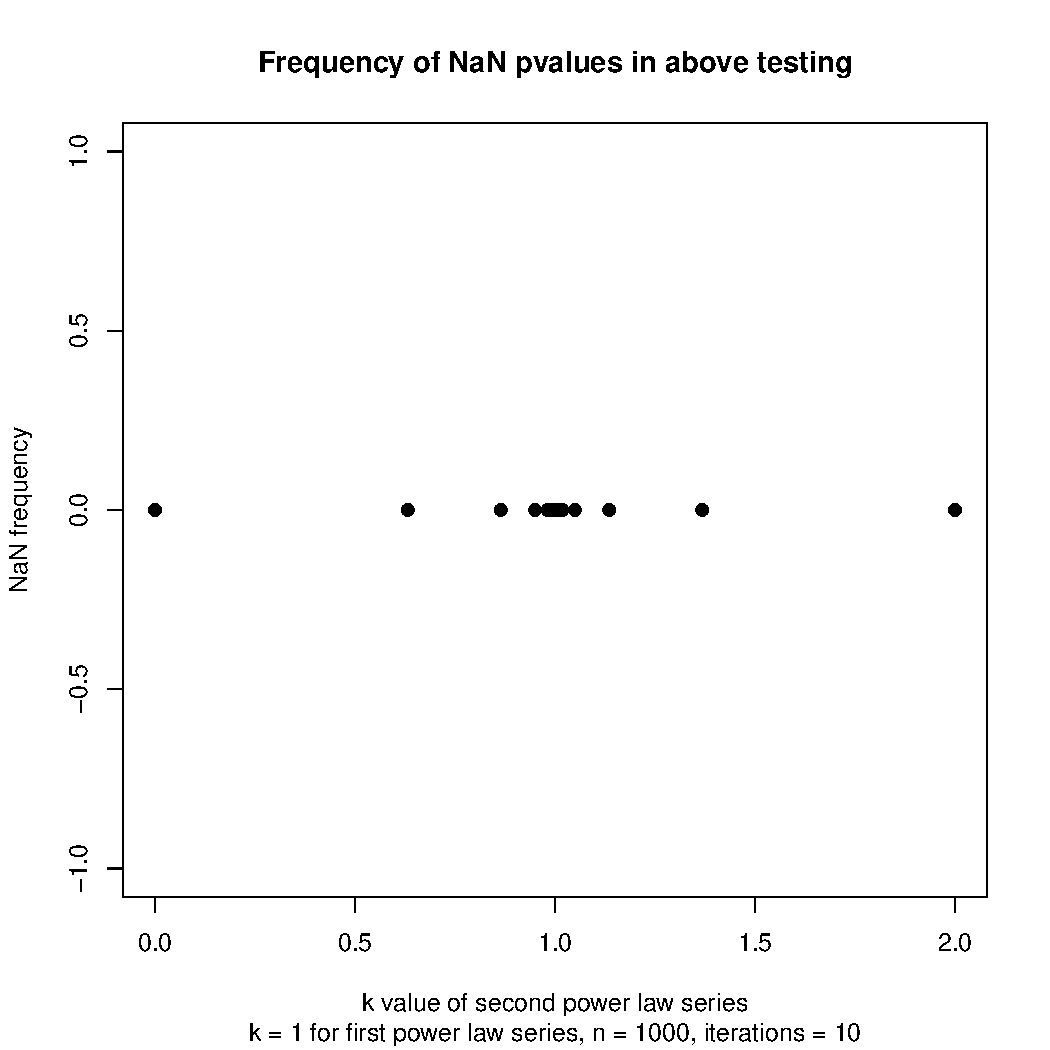
\includegraphics[height=7cm,keepaspectratio]{powerlaw/NaNPlot,k1=1, n=1000, iterations=10.pdf}
    \end{subfigure}
    \vfill
    \begin{subfigure}[b]{0.3\textwidth}
        \centering
        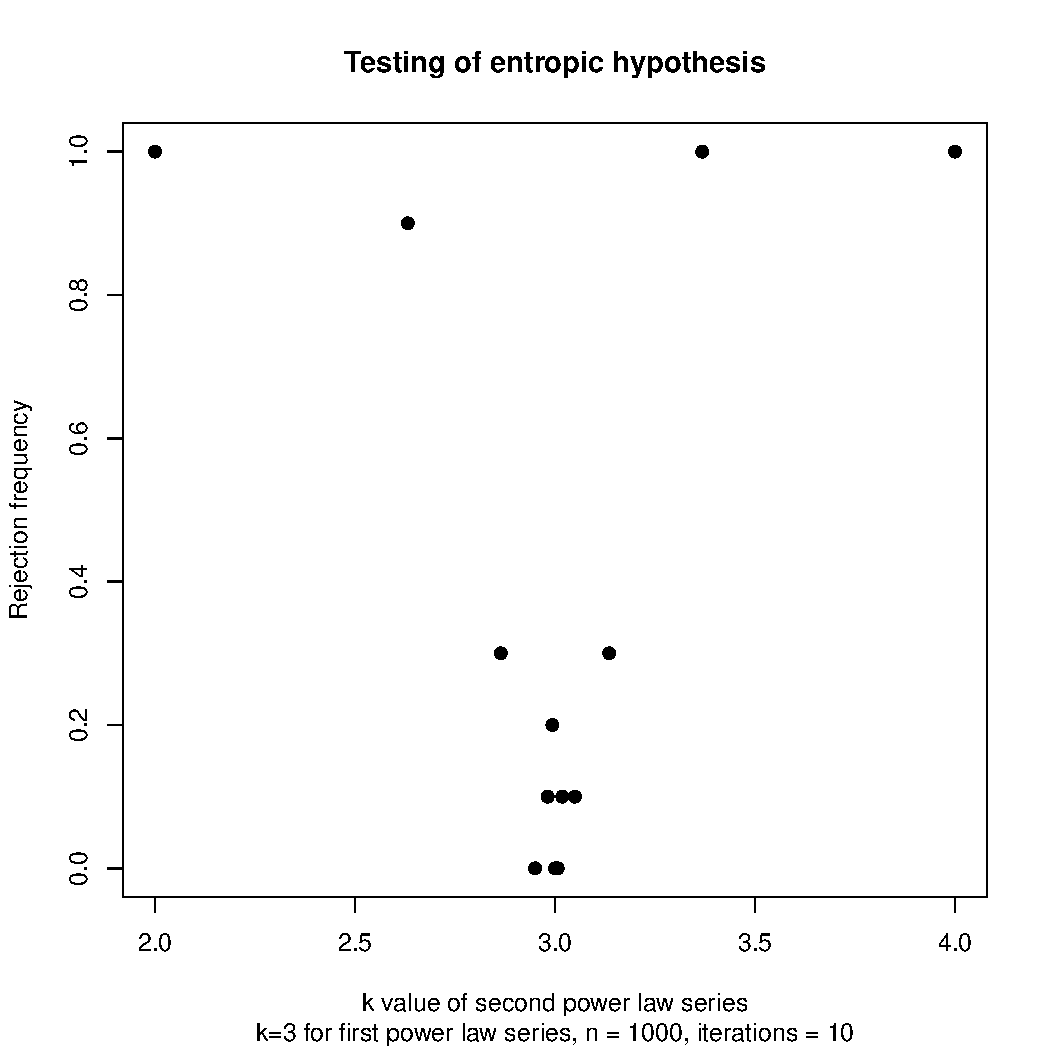
\includegraphics[height=7cm,keepaspectratio]{powerlaw/rejectionPlot,k1=3, n=1000, iterations=10.pdf}
    \end{subfigure}
    \hfill
    \begin{subfigure}[b]{0.5\textwidth}
        \centering
        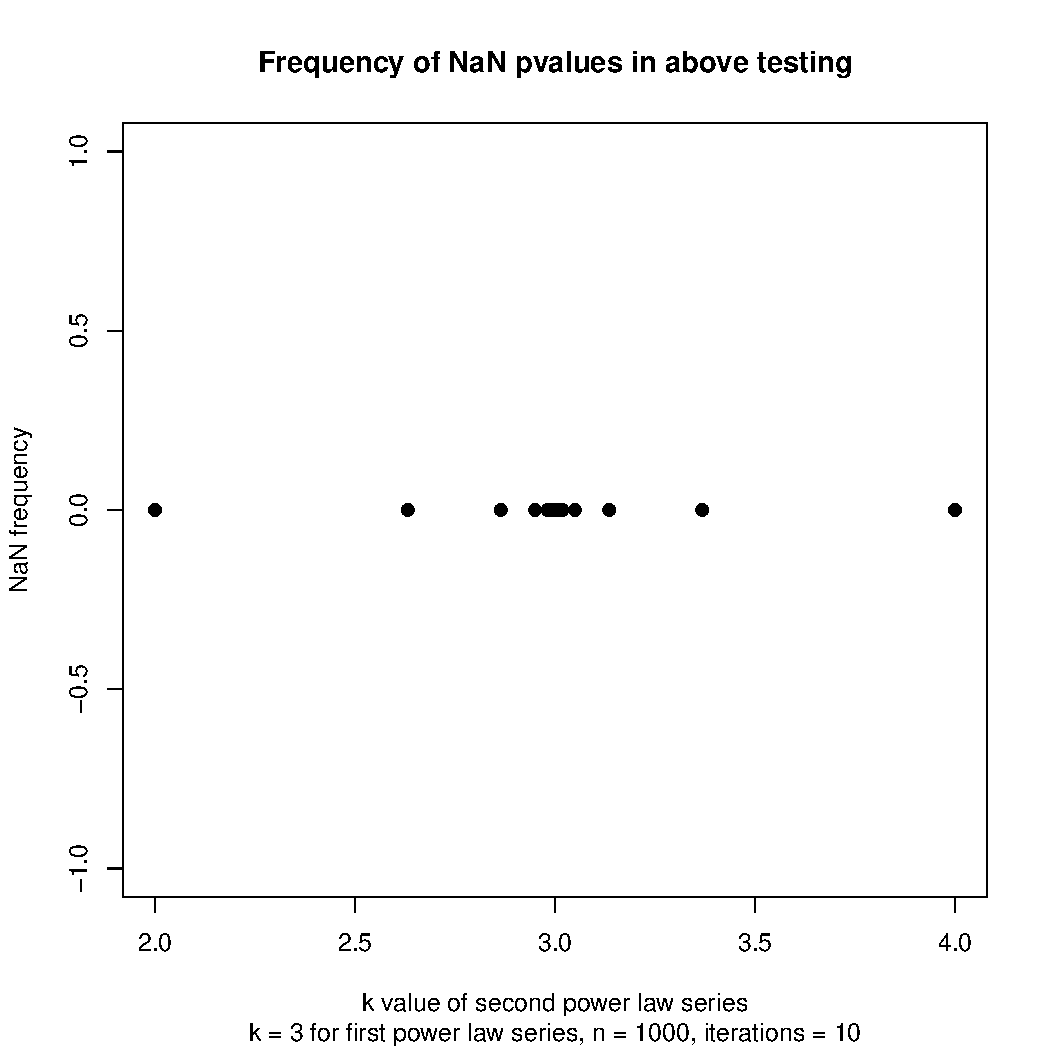
\includegraphics[height=7cm,keepaspectratio]{powerlaw/NaNPlot,k1=3, n=1000, iterations=10.pdf}
    \end{subfigure}
    \vfill
    \begin{subfigure}[b]{0.3\textwidth}
        \centering
        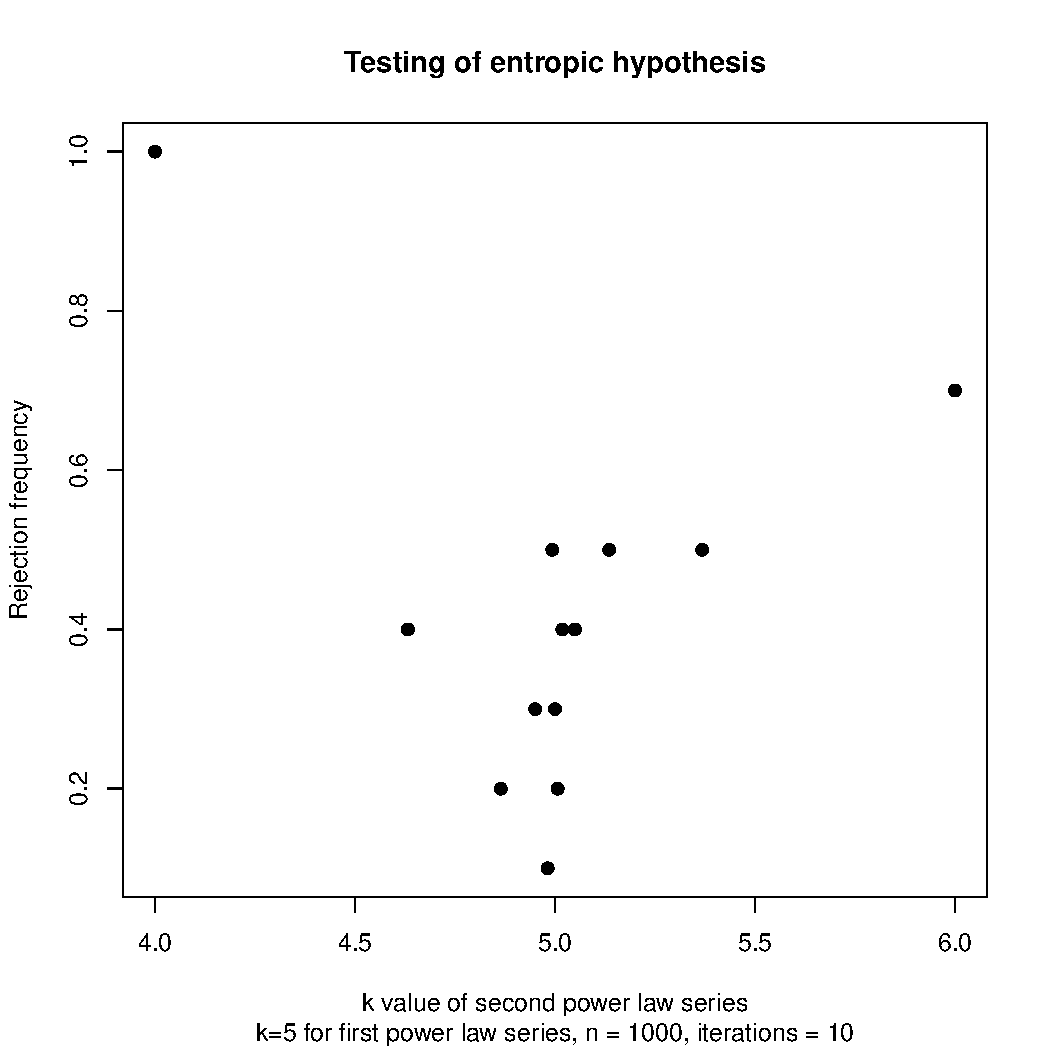
\includegraphics[height=7cm,keepaspectratio]{powerlaw/rejectionPlot,k1=5, n=1000, iterations=10.pdf}
    \end{subfigure}
    \hfill
    \begin{subfigure}[b]{0.5\textwidth}
        \centering
        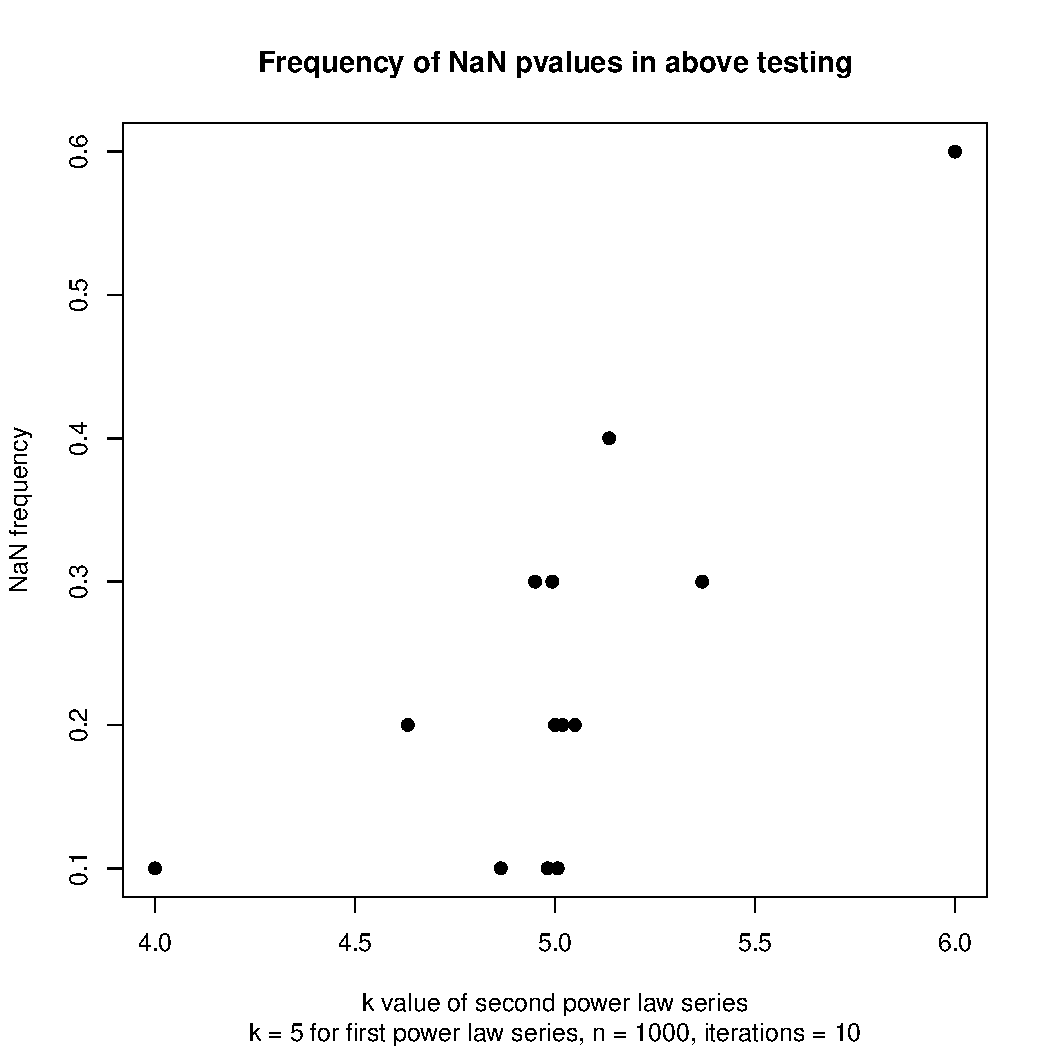
\includegraphics[height=7cm,keepaspectratio]{powerlaw/NaNPlot,k1=5, n=1000, iterations=10.pdf}
    \end{subfigure}
    \caption{Power-law experiment}
\end{figure}

\FloatBarrier

\paragraph{Idea behind new tie breaking}
In the next section a new way to break ties will be implemented and used. The idea behind it is, when having a tie, instead of either randomly assigning it to any of the possible patterns, which was proposed by bandt and pompe in their original paper \cite{Bandt2002}, or always assigning a type of tie to a given pattern, which is done in the article being used in the next section \cite{Chagas2022}. The new idea is to assign an equally large weight to all the possible patterns in case of a tie. In a tie, with k possible patterns, that it could be, each of these k patterns gets a weight of $\frac{1}{k}$. The amount of possible patterns is the product of the occurrence of each unique value. In case of a non-tie the pattern gets weight 1. To calculate the ordinal pattern distribution simply sum up all the weights for each pattern and divide by total amount of weight to get frequency. Ordinal patterns is often used in fields that does science on real world phenomenons. In cases where the measuring equipment has a low precision ties will often occur e.g. a weight measurement. It is commonly known that objects have an atomic weight, since all everyday objects is made of particles that have an atomic weight. $1\mu = 1.66..\cdot10^{-27}kg$, so the theoretical weight of an object has a lot of decimals, which could theoretical be measured, however putting a person on a normal household weight  will only give a result in kilograms with one decimal. A person measuring themselves on a weight at different and weighing the same does not mean they had the same atomic weight at both times. Their data would result in a tie, but based on the above argumentation it is fair to assume that in reality the weight has either gone up or down, however it is impossible with the given instruments to measure, which it is, so the only fair assumption is that both cases is equally likely. This can almost be seen as superposition\cite{Schroedinger1926} of the change of weight. The weight has gone both up and down, until a more precise measurement is made, but until that it is only fair to think both cases possible and in this case equally possible. This type of tie breaking should work, where it can be argued that a theoretical measurement has a higher precision that the actual measurement. It does however not make sense to use in when the measured value can be argued to be of the same precision of a theoretical measurement e.g. "how many cows are out on the field at a certain type?". This implementation will briefly be referenced "My implementation", but mostly as "Theoretical Split". Note that the theoretical split method does not need noise added. Adding noise removes all ties, which means it should perform identical to "article implementation", which is the implementation made in the article\cite{Chagas2022}, since it is built upon that code. The theoretical split and the second tie breaking solution is deterministic, where the bandt and pompe solution is stochastic.

\FloatBarrier

\paragraph{Temperature Data}
\cite{Chagas2022} Will be partly reproduced and additional plots and tables will be made. Only the maximum temperature part of the climate data in section 6 of the article will be used. As can be seen in figure 3.2 the percentage of ties in this dataset is extremely high. It is therefore quite important, how ties is handled, since they make up a bulk of the dataset. 
\begin{figure}
    \centering
    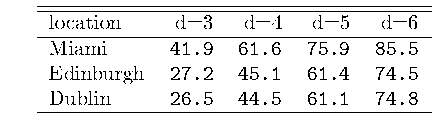
\includegraphics{Weather/tiesTable.pdf}
    \caption{Table of ties in percentage}
\end{figure}


The libraries mentioned earlier all handle ties differently as can be seen in figure 3.3. The first three columns is the setting of each experiment. The start date column is included, because the paper, where the data is from, accidentally started their data at 1992-08-14, instead of 1992-08-08 as they said the data started from, it does however not make a big difference, which can be seen between the top three rows and bottom three rows.  If all the values in a row is identically that means the libraries perform identically. The only setting, where this happens is when noise is added and Na values is omitted. Na omit removes Na values and the dataset is pushed together, where the Na values have been removed. In the rest of the experiment this setting will be used. 

\begin{figure}
    \centering
    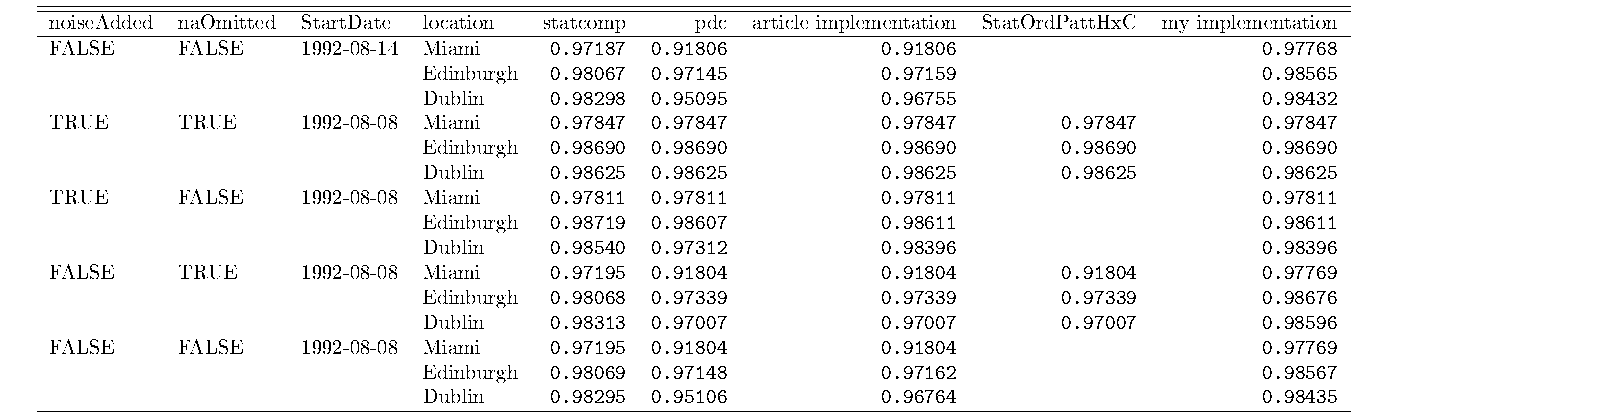
\includegraphics[width=\textwidth,keepaspectratio]{Weather/entropyTable.pdf}
    \caption{Entropy table of libraries performs on different preprocessing}
\end{figure}

A more in depth analysis of the Theoretical Split vs adding noise is made. The statcomp library is the comparison library, but it does not matter, which library is chosen, since they perform identical in this case. As it can be seen in figure 3.5 the theoretical value is very close to both the mean and median of the entropy of a 1,000 iterations. Figure 3.4 clearly shows the problem of adding a random sample of white noise, since the value might easily end up 0.001 off either the mean, median or theoretical value, which all seems to quite precise values of the entropy, since the theoretical value is calculated quite differently then the mean and median, but they still end up much closer, then a random sample do. 

\begin{figure}
    \centering
    
\includegraphics[width=\textwidth,keepaspectratio]{Weather/noiseStochasticTheoretical.pdf}
    \caption{Iterations of adding noise vs theoretical split in sorted order, vertical line is median and horizontal is theoretical split value.}
\end{figure}

\begin{figure}
    \centering
    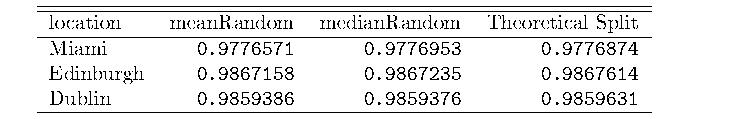
\includegraphics[width=\textwidth,keepaspectratio]{Weather/random_vs_theoreticalSplit.pdf}
    \caption{Table of: mean and median of adding noise and theoretical split. Temperature dataset}
\end{figure}

The above experiment is repeated, but where the theoretical split is fed a constant dataset. The constant values here represent very imprecise measurements, where the true values of the observed phenomenon is assumed to be different. E.g. trying to measure white noise, with a bad instrument. It is important to note that, if a dataset contained just a single constant value, where the measurement is precise. The entropy would naturally be 0, since there is full predictability e.g. "how many cows are on the field at a given time". The iterations is calculated on random numbers, which ideally should be white noise. Figure 3.6 rarely has the entropy of ideal white noise, which is 1, where the theoretical split is able to correctly calculate that the poorly measured white noise has entropy 1. Figure 3.7 shows that the median measurement is closer then the mean to the theoretical split, so it might be a better measurement. In figure 3.5 the median is generally also closer to the theoretical split. The median has another benefit over the mean, in the fact that it might not always be mathematically true to take the mean of an approximation, where the median is an entropy generated by an actual time series.

\begin{figure}
    \centering
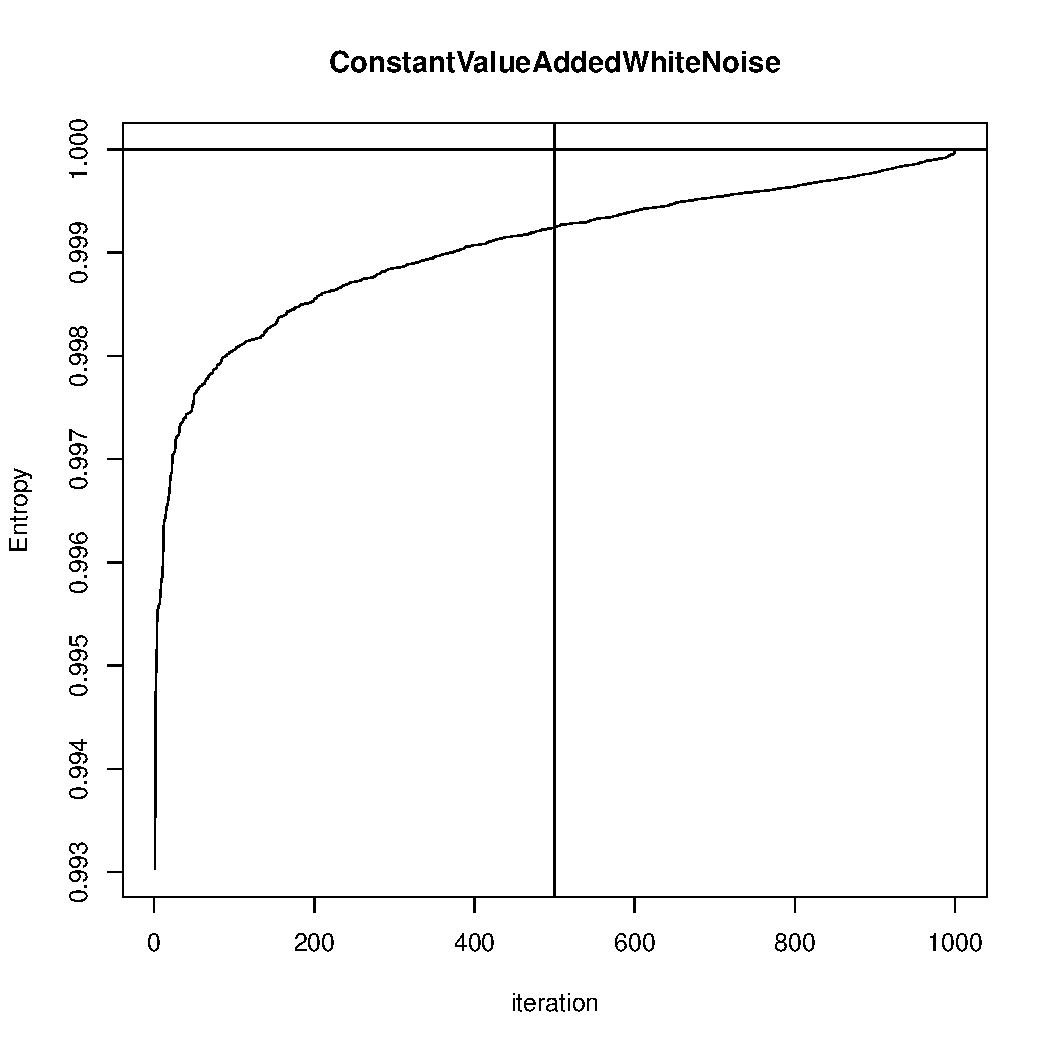
\includegraphics[width=\textwidth,keepaspectratio]{Weather/constantWithWhiteNoiseStochasticTheoretical.pdf}
    \caption{Constant dataset}
\end{figure}

\begin{figure}
    \centering
    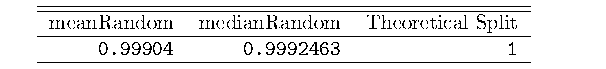
\includegraphics[width=\textwidth,keepaspectratio]{Weather/random_vs_theoreticalSplitWhiteNoise.pdf}
    \caption{Mean and median of adding noise and theoretical split, constant dataset.}
\end{figure}

Figure 3.8 is a plot of the theoretical split values as entropy of the three locations on the HxC plane with confidence intervals on the entropy. In this case, the confidence intervals sticks out of the boundaries of the HxC plane. Between the boundaries is the only area where it is possible for a time series to be plotted. In this case the confidence interval do not offer new information, however it would be interesting to plot it, when the entropy is around 0.5, since the boundaries is much futher apart.

\begin{figure}
    \centering
    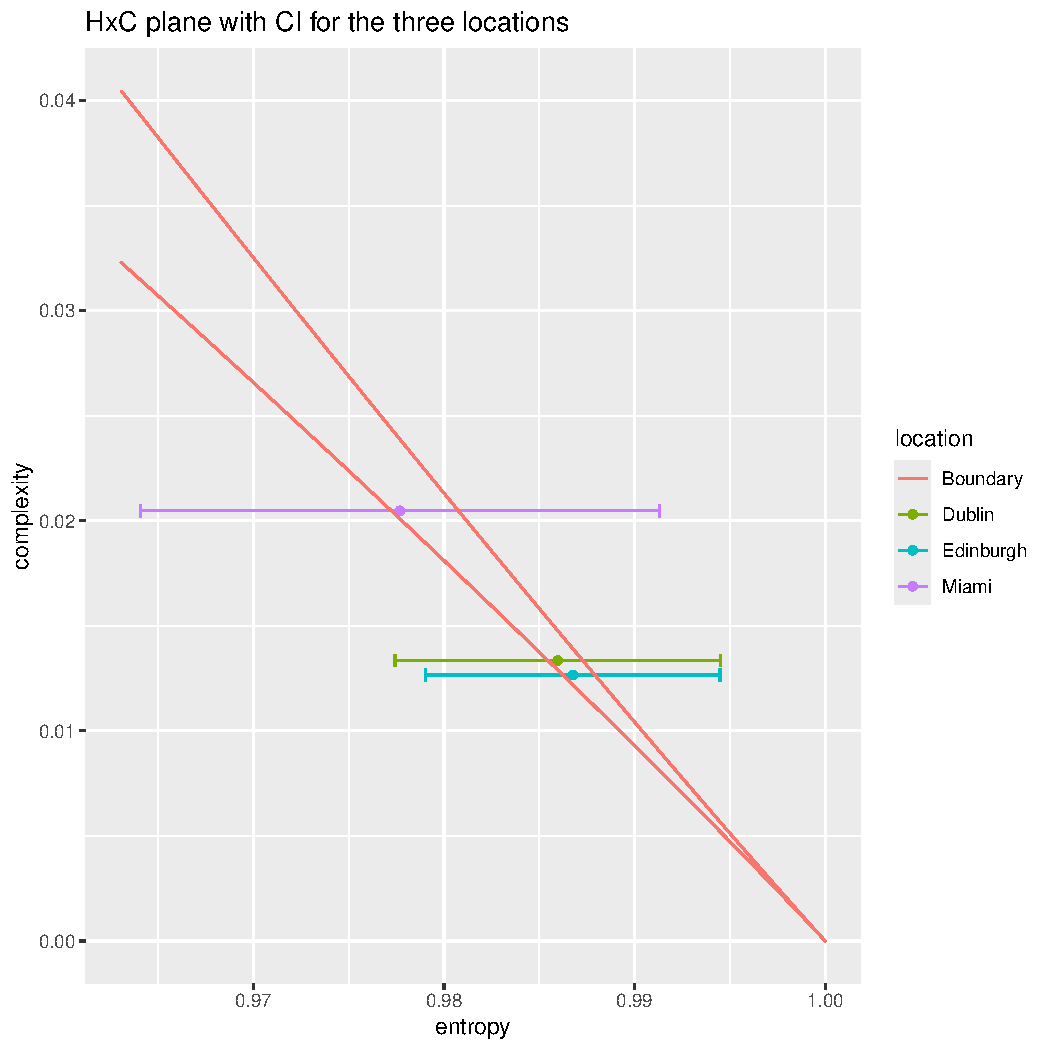
\includegraphics[width=\textwidth,keepaspectratio]{Weather/confidenceIntervalPlot.pdf}
    \caption{HxC plane of locations with confidence interval}
\end{figure}

P values is calculated. 10 iterations is done on adding noise for breaking ties and compared with the p value of the theoretical split. The p values of the theoretical split is in between the two median values, for Edinburgh-Dublin, which is good. For Miami-Edinburgh it is the second largest value, which is worse, however still in the interval of the iterations. For Miam-Dublin three iterations gets larger p values then the theoretical, which is ok. The theoretical split method produces p values that are reasonable close to the iterations of adding noise. Adding noise has a couple of problems in the sense that it is much more computer intense to calculate just 10 iterations compared with the theoretical value once.
'\begin{figure}
    \centering
    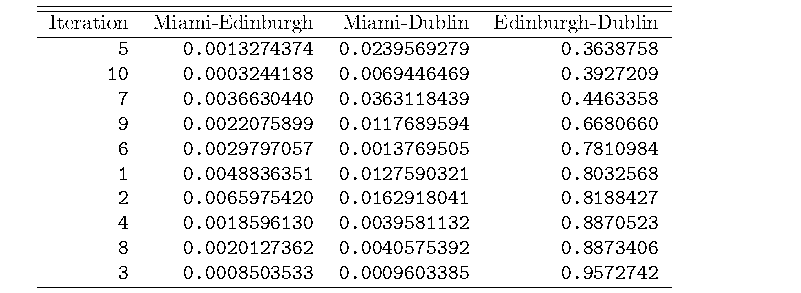
\includegraphics[width=\textwidth,keepaspectratio]{Weather/pValuesTheoretical,10=Iterations,Sorted.pdf}
    \caption{Noise added, 10 iterations, sorted by column "Edinburgh-Dublin"}
\end{figure}

'\begin{figure}
    \centering
    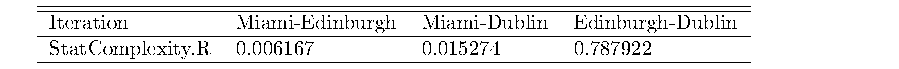
\includegraphics[width=\textwidth,keepaspectratio]{Weather/pValuesTheoretical.pdf}
    \caption{p value, when using theoretical split}
\end{figure}

